\subsubsection{Aktualizacja systemu}
\label{rzeczy_do_zrobienia_po_instalacji}
\begin{wrapfigure}{R}{0.1\textwidth}
        
\includegraphics[width=\linewidth]{images/pierwsze_uruchomienie_aktualizacja1.png}
\end{wrapfigure}

Kliknij na ikonę Dash 
\includegraphics[scale=0.35]{images/ikony_dash.png} i wpisz "Aktualizacje". W czasie wpisywania na ekranie wyników będą się pojawiały propozycje. Z wiersza "Programy" wybierz "Aktualizacje oprogramowania".
System sprawdzi, czy dostępne są aktualizacje dla twojego Ubuntu i wyświetli podsumowanie.
\begin{center}
        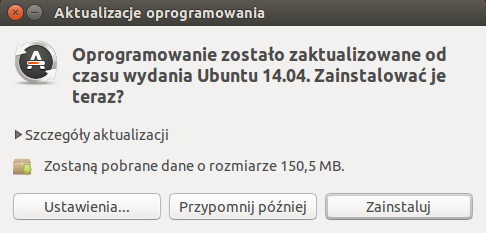
\includegraphics{images/pierwsze_uruchomienie_aktualizacja2.png}
\end{center}

Kliknij na przycisk \textcolor{ubuntu_orange}{Zainstaluj} aby zainstalować aktualizacje. Zostaniesz poproszony o podanie hasła w celu uwierzytelnienia. Każda operacja mająca wpływ na cały system wymaga potwierdzenia. Zapobiega to przypadkowemu uszkodzeniu systemu.
\begin{center}
        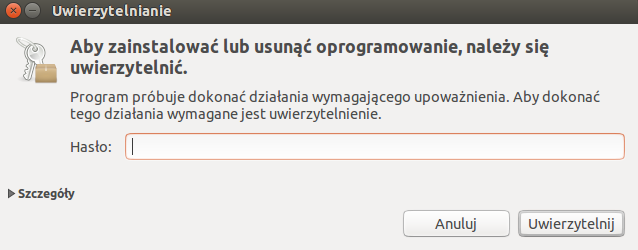
\includegraphics{images/unity_uwierzytelnienie.png}
\end{center}

Wpisz swoje hasło i potwierdź klawiszem Enter, lub kliknij na przycisk \textcolor{ubuntu_orange}{Uwierzytelnij}. Teraz rozpocznie się proces pobierania i instalacji aktualizacji. Proces ten może potrwać od kilkunastu sekund do kilku minut, w zależności od tego jak dawno system nie był aktualizowany.

Kiedy aktualizacja się zakończy możesz zostać poproszony o zrestartowanie komputera. Restart jest potrzebny tylko jeżeli aktualizowane było jądro systemu lub sterowniki. Inne aktualizacje nie wymagają restartu komputera a jedynie restart zaktualizowanego programu.

W przyszłości system będzie automatycznie sprawdzał czy dostępne są aktualizacje i powiadomi cię o tym.

\subsubsection{Instalacja spolszczenia}
\begin{wrapfigure}{R}{0.1\textwidth}
        
\includegraphics[width=\linewidth]{images/pierwsze_uruchomienie_lang1.png}
\end{wrapfigure}

Jeżeli w trakcie instalacji systemu nie wybrałeś języka Polskiego lub nie miałeś połączenia z internetem aby ściągnąć potrzebne paczki językowe to tutaj dowiesz się jak zainstalować odpowiednie oprogramowanie.
Kliknij na ikonę Dash 
\includegraphics[scale=0.35]{images/ikony_dash.png} i wpisz \textcolor{ubuntu_orange}{Języki}. System sprawdzi stan spolszczenia systemu i zaproponuje instalację dodatkowych paczek. Kliknij \textcolor{ubuntu_orange}{Zainstaluj} a następnie potwierdź operację. Wpisz swoje hasło i potwierdź klawiszem Enter, lub kliknij na przycisk \textcolor{ubuntu_orange}{Uwierzytelnij}.
\begin{center}
        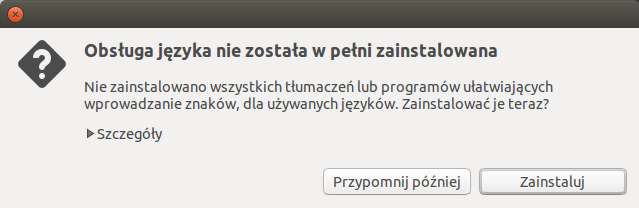
\includegraphics{images/pierwsze_uruchomienie_lang2.png}
\end{center}

Po instalacji niezbędnych paczek możesz jeszcze dla pewności kliknąć na \textcolor{ubuntu_orange}{Zastosuj dla całego systemu}. Aplikacja upewni się w ten sposób, że cały system został spolszczony.
W przyszłości aplikacja \textcolor{ubuntu_orange}{Języki} pozwoli ci w łatwy sposób zainstalować i zmienić język systemu na każdy z wspieranych przez społeczność Ubuntu.

\subsubsection{Instalacja dodatkowych sterowników}
\begin{wrapfigure}{R}{0.1\textwidth}
        
\includegraphics[width=\linewidth]{images/pierwsze_uruchomienie_driver1.png}
\end{wrapfigure}

Prawdopodobnie nie wszystkie sterowniki zostały włączone podczas instalacji Ubuntu. Aby się upewnić, że sprzęt jest prawidłowo obsługiwany Kliknij na ikonę Dash 
\includegraphics[scale=0.35]{images/ikony_dash.png} i wpisz \textcolor{ubuntu_orange}{Sterowniki}. Z wyświetlonych wyników wybierz "Aktualizacje i sterowniki. W otwartym oknie przejdź na zakładkę "Dodatkowe sterowniki". Poczekaj chwilę aż system zbierze dane o twoim komputerze i porówna je z bazą danych sterowników. Z wybranej listy będziesz mógł wybrać, który sterownik powinien zostać użyty.
\begin{center}
        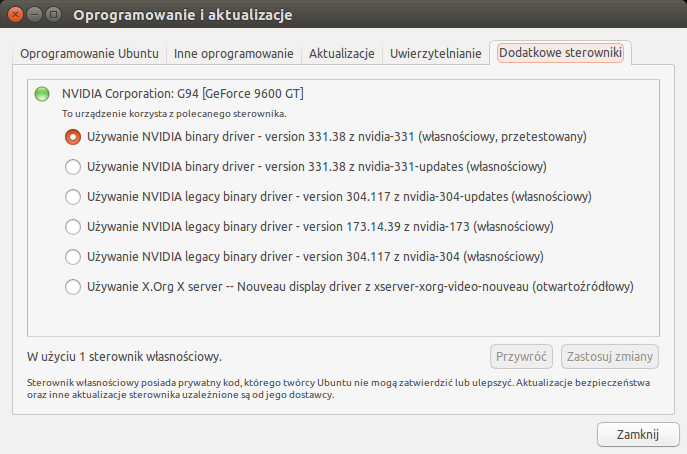
\includegraphics[width=\linewidth]{images/pierwsze_uruchomienie_driver2.png}
\end{center}

Zmiana sterownika wymaga potwierdzenia. Wpisz swoje hasło i potwierdź klawiszem Enter, lub kliknij na przycisk \textcolor{ubuntu_orange}{Uwierzytelnij}. Więcej o wyborze sterownika przeczytasz w rozdziale \ref{sterowniki}: Sterowniki

\subsubsection{Instalacja dodatków}
\begin{wrapfigure}{R}{0.1\textwidth}
        
\includegraphics[width=\linewidth]{images/pierwsze_uruchomienie_dodatki1.png}
\end{wrapfigure}

Na koniec warto zainstalować kilka pakietów oprogramowania Kliknij na ikonę Dash 
\includegraphics[scale=0.35]{images/ikony_dash.png} i wpisz \textcolor{ubuntu_orange}{Centrum Oprogramowania}. Z wiersza \textcolor{ubuntu_orange}{Programy} wybierz \textcolor{ubuntu_orange}{Centrum Oprogramowania Ubuntu}. W prawym górnym rogu nowo-otwartego okna masz wyszukiwarkę. Wpisz w nią \textcolor{ubuntu_orange}{Ograniczone dodatki Ubuntu} i wciśnij enter. Poczekaj aż odnaleziona zostanie ta paczka. Z listy wybierz \textcolor{ubuntu_orange}{Ubuntu restricted extracts} i kliknij \textcolor{ubuntu_orange}{Zainstaluj}. Instalacja oprogramowania wymaga uwierzytelnienia. Wpisz swoje hasło i potwierdź klawiszem Enter, lub kliknij na przycisk \textcolor{ubuntu_orange}{Uwierzytelnij}.
\begin{center}
        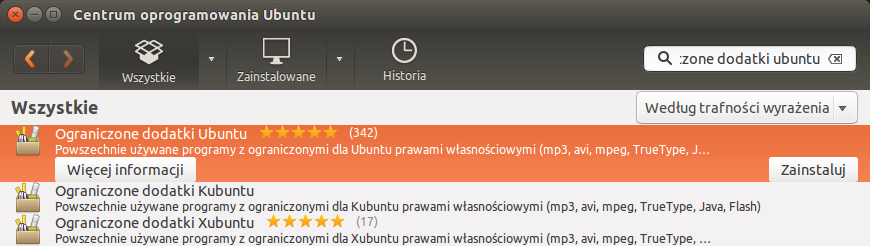
\includegraphics[width=\linewidth]{images/pierwsze_uruchomienie_dodatki2.png}
\end{center}

Paczka \textcolor{ubuntu_orange}{ubuntu-restricted-extras} zawiera w sobie:
\begin{itemize}
\item Wszystkie możliwe kodeki audio/wideo.
\item Odtwarzcacz Flash.
\item Java.
\item Fonty True Type (np. Times New Roman).
\end{itemize}
W podobny sposób wyszukaj i zainstaluj programy \textcolor{ubuntu_orange}{openjdk-7-jre}(Java, potrzebna do wielu popularnych programów), \textcolor{ubuntu_orange}{unzip} (obsługa archiwów zip) i \textcolor{ubuntu_orange}{p7zip-full} (obsługa archiwów w formacie 7z/lzma).
\clearpage
